\documentclass{report}
%Math Stuff
\usepackage{amsmath}
\usepackage{enumitem}
\usepackage{mathtools}

%General Formating
\usepackage[letterpaper, portrait, margin=1in]{geometry}
\usepackage{fancyhdr}
\pagestyle{fancy}

%Bibliography
\usepackage[toc,page]{appendix}
\usepackage{hyperref}

%Figures
\usepackage{graphicx}
\graphicspath{ {figures/} }
\usepackage{tikz}
\usepackage{pgfmath}
\usepackage{framed}
\usepackage{csvsimple}
\usepackage{rotating}
\usepackage[section]{placeins}

%Header
\lhead{Schulman}
\rhead{Page \thepage}

%Title
\title{Food Networks \\~\\ \normalsize A Thesis Presented to the Faculty of the Economics Department of Cornell University in Partial Fulfillment of the Requirements for the Degree of Bachelor of Arts in Economics with Honors} 
\author{Eric Schulman}
\date{May 2017}

\begin{document}

\maketitle

\pagebreak

\begin{abstract}
For my thesis, I ask how the network of farms, intermediaries and stores involved with agricultural production relates to prices and nutrition. Suppliers incur transportation costs while navigating products from farms to stores. Considering the difficulty involved with finding statewide data on prices, estimating these costs provides the best possible insight into the prices consumers face at stores. To estimate transportation costs at stores, I track the supply of grapes, cabbage, onions and cherries as it moves from farms to stores in New York state using data from satellites and public records. Using this data, I estimate the least costly path for transporting the goods from the farms to the stores using a linear programming software package. According to my estimates, transporting produce to the northeast and southeastern parts of the state is most expensive. Additionally, when the farms vary in size, the cost of sending produce to stores gets noticeably amplified in the optimal solution. All of the code to used to complete this project is publicly available on GitHub at \url{http://github.com/erichschulman/ag_networks}. 
\end{abstract}

\pagebreak

\renewcommand{\abstractname}{Acknowledgments}
\begin{abstract}
This has been an incredible experience and I've learned so much! I couldn't have done this project without the tremendous amount of support I've gotten from the faculty in the department of economics. I want to explicitly thank Professor Patacchini for advising the project and Professor Besharov for running the honors program. I also want to thank Professor Tardos in computer science for helping me to understand the algorithms involved with this project and Professor Easley and Professor Caunedo for their feedback over the past few months. 
\end{abstract}

\tableofcontents

%background
\chapter{Introduction}
\section{Background}

Economics and nutrition are no strangers to each other. Economists and other social scientists have tried to explain and improve nutritional outcomes for years. The literature calls adequate nutritional outcomes food security. Food security consists of three dimensions: availability, accessibility and utilization. Availability reflects whether food is available in stores. Access reflects whether individuals can afford it. Utilization reflects what individuals do with food after buying it \cite{barrett}. In the past, researchers measured food security using a questionnaire about nutritional practices. The questionnaire asks respondents whether they purchased vegetables, ate three meals each day and similar questions. Responses to the questionnaire reflects levels of food security.

For a long time, researchers explained the answers to surveys about food security using the answers' statistical relationship with transfer programs and demographics. The United States publishes a survey about food security each month called the CPS nutritional supplement. Demographic information about participants in the nutritional supplement gets tracked as part of the regular CPS. Calculating the statistical relationships between the survey and factors like race, income and education is straightforward.

This literature finds that reducing costs and increasing availability of nutritional foods improves health outcomes. One study evaluated the Farmers' Market Nutrition Program, a national program intended to increase consumption of fresh fruits and vegetables by providing coupons and information. Researchers found subsidizing nutritionally rich food with coupons leads to increased consumption when complemented with information \cite{Just}. Researchers also began noticing the statistical importance of systemic factors in determining nutritional outcomes. For example, researchers analyzed nutritional outcomes in Oregon between 1999 and 2001, when Oregon had the highest average rate of hunger in the nation. The study found factors like residential location and housing costs were most related to food insecurity \cite{Bernell}.

In recent years, social scientists have placed a lot of importance these factors in determining nutrition. They began studying nutritional habits in the context of individuals' environments. Instead of trying to measure the statistical relationship between a family or individual characteristics with eating outcomes, the researchers classify environments that put individuals at risk to be unhealthy based on factors like high prices or limited access to fresh produce. Most studies call areas where residents have difficulty maintaining a balanced diet food deserts. The term originated to describe public housing developments in western Scotland with a limited number of grocery stores and other options for nutritious foods. Especially in the past five years, this term has captured the imagination of policy makers in the United States.

A lot of research has been focused on finding and classifying food deserts. These studies leverage spatial coordinates and mapping software to find regions that discourage healthy nutritional outcomes based on regions' proximity to grocers and prices. One study conducted in the twin cities area focused on prices and concluded that the urban poor pay marginally more for food. Often times, food is cheaper at supermarket chains, but these stores are hard to find in inner cities \cite{Chung}. Many studies augment their observations using demographic information. Another study conducted in the twin cities area used directories of grocery stores combined with demographic information to index neighborhoods' vulnerability to food insecurity \cite{Larson}. In another project, researchers leveraged Google Maps and local online news to build a graphical representation of food availability in Bogota, Columbia \cite{Hwang}. 

The literature on food deserts focuses on observing the locations of food suppliers and prices to identify food insecurity. It generally ignores the endogenous factors that determine the placement of stores or prices even though researchers in the field of operations research have studied how suppliers decide on the allocation of food. Food allocation is often studied using a transportation problem. Transportation problems are an optimization problem designed to find the cheapest possible way of sending a certain amount of supply through a network. It can be solved efficiently using the network simplex algorithm and linear programming software packages \cite{Cook}. Researchers often apply transportation problems to food allocation. One paper studied maize allocation in South Africa where trains carry maize from supply and demand points, scattered throughout the country. Researchers minimize the total rail cost, as is standard, but add a secondary objective of distributing costs fairly among all users \cite{Stewart}.

\section{Research Question} 

For my project, I tried to answer how the network of farms, stores and intermediaries impacts the price of purchasing fresh produce in New York State. Following much of the nascent literature on food deserts, I use spatial data and demographic information to identify regions where the structure of food distribution makes purchasing certain types of produce difficult. Specifically, I tracked the movements of onions, cherries, grapes and cabbages across New York state and leveraged the operations research literature regarding the optimal allocation of food to estimate their transportation costs as they move through their supply chain from farms to stores. 

My analysis of transportation costs has the same intentions as the existing literature on food deserts, but my perspective is different. I also try to identify regions with limited access to produce due to high costs. However, instead of thinking about nutrition in terms of food deserts, my project is about food networks. In other words, instead of using the isolated characteristics of certain areas to predict troubling nutritional outcomes, I predict outcomes using connections between areas. 

By focusing on the relationship between the nutritional characteristics of different regions, I improve the literature in two ways. First, most studies look at regions in isolation by focusing on demographics and regions' proximity to stores. However, records about the locations of stores do not exist in rural areas causing them to be overlooked. By focusing on how onions, cherries, grapes and cabbages move through the supply chain, I can provide insight into prices across the state. This insight is limited to these types of produce, but it may be indicative of produce in general. Secondly, the existing literature often ignores how endogenous factors contribute to nutritional outcomes in food deserts. By focusing my attention to tracking a few crops through the overall supply network contribute to prices, I address the interacting considerations of suppliers in determining supply.

\section{Economic Mechanism}

In order to predict where produce was expensive for consumers, I tracked the supply chain of cherries, cabbages and onions in New York state using satellite data and public records. Using this data, I estimate the transportation cost associated with moving produce from farms to stores. In order for transportation costs to predict prices the other factors involved with determining prices must be relatively similar across suppliers. Since the crops I chose are not produced on a large scale, the factors involved with production are similar. Suppliers face similar demand because in the short term, prices are sticky. For example, even if a grocery store does not sell onions on a given day, prices will stay the same. All this to say, with the exception of transportation costs, supply and demand for produce is similar over a small region like New York. Over the long run, firms and consumers can move. As a result, transportation have weight in predicting prices. This in turn, impacts nutrition considering the link between prices and nutritional outcomes in the literature. 

Focusing on crops with a short shelf life, produced on a small scale makes tracking their supply chain simple. With the exception of grapes, New York produces limited quantities of onions, cherries and cabbages as you can see from Table \ref{tab:nass3}. Cabbage, onions and cherries have short shelf lives discouraging the crops from being sold out of state as you can see in Table \ref{tab:nass2}. This table compares production of these crops to the amount of these crops that are sold for USDA organic crops \cite{nass2}. Because production is small, it largely falls into three stages. First, farms produce crops. Then they send their crops to intermediaries called agricultural dealers. The dealers may bag the produce but mostly facilitate its movement between farms and stores. After agricultural dealers send the produce to stores, stores sell the crops to consumers. New York state releases data on each of the stages of this process. Specifically, my data contains the size and location of farms, the location of dealers and the size and location of stores. 

Since the crops are sent directly from farms to dealers to stores, I know where the crops are at each stage in their supply chain. I do not know how produce moves between stages, but it seems reasonable to assume farms chose where to send their produce in such a way that keeps costs as low as possible. Building on the assumption that farms, dealers and stores try to minimize the of moving produce through the network, I can fill in the missing pieces about how produce moves between the farms, dealers and processors by optimizing the movements of crops based costs. By optimizing the transportation costs through this network, my project incorporates the literature that treats agricultural markets as an optimization problem. 

The inputs to the problem involve the quantities of produced at farms and sold at stores. Capacities of farms and stores and transportation costs are determined endogenously. For example, farms may grow more produce if stores are nearby. Although this is important, it is safe to treat these inputs as fixed in the short run because agriculture is capital intensive. Because of high fixed costs, new farms and stores cannot constantly enter the market. More over, once farms buy land and equipment, the amount they produce over the course of a season will not change because a store with low transportation costs opens nearby. Stores have an easier time scaling if new nearby farms with low transportation costs enter the market. However, their floorspace is static and it takes time for farms to start growing. Also financial contracts requiring stores to purchase produce get set before the growing season.

\begin{table}[!t]
\centering
\begin{framed}
\begin{tabular}{c|c|c|c}%
	Item&Sales (1000 USD)&Rank by Sales&Percent of Total Sales
    \csvreader[head to column names, /csv/separator=semicolon]{nass3.csv}{}% use head of csv as column names
    {\\\hline \csvcoli & \csvcolii & \csvcoliii & \csvcoliv}
\end{tabular}
\caption{This table shows various crops in New York state. Fresh produce (labeled as Fruits and Vegetables) makes up about $10 \%$ of New York's agricultural sales \cite{nass3}.}
\label{tab:nass3}
\end{framed}
\end{table}

\begin{table}[!t]
\centering
\begin{framed}
\begin{tabular}{c|c|c|c|c}%
	Crop&Total Production (CWT)& Fresh Market Sales (CWT)&Percentage&Year
    \csvreader[head to column names, /csv/separator=semicolon]{nass2.csv}{}% use head of csv as column names
    {\\\hline \csvcoli & \csvcolii & \csvcoliii & \csvcoliv& \csvcolv}
\end{tabular}
\caption{This table compares the organic production of onions, grapes, and cabbages in New York to the amount that is sold on the fresh market \cite{nass2}. The amount produced and sold is measured in hundredweight (CWT). For perspective, about seventeen CWT make up one US ton. I chose 2011 as the year because that was the year the crop cover data was produced. The these crops are USDA organic meaning that they do not represent all production. Organic cherries are produced in such limited quantity in New York that their production isn't included in the data.}
\label{tab:nass2}
\end{framed}
\end{table}

\chapter{Linear Model}

\section{Model Overview}

The optimization problem of minimizing transportation costs while ensuring markets clear is called optimal transportation. Some call it minimum-cost flow because the objective involves maximizing the amount of flow (in my case, units of produce flowing through the network of farms, stores and intermediaries) at the minimum cost. If you are familiar with matching markets and augmenting paths, minimum-cost flow will seem familiar because minimum-cost flow is a more general version of a matching market. You can use the augmenting path algorithm for matching markets to solve the problem. You start by using augmenting paths to find the maximum amount of flow through the network. Then you try to optimize cost by starting at a supply node and finding cycles that alternate between supply and demand while reducing cost. Describing the problem with words is much harder than working out a visual example. For this reason, I included a manageable example of a transportation problem with a network of two suppliers and three consumers in Figures \ref{fig:example1} through \ref{fig:example6} in the appendix. Following the example will clarify the problem's nature and how to solve it.

For my project, I apply minimum-cost flow to agricultural markets in New York to estimate shipping costs from data about supply and demand for produce. In the network, farms can ship to any intermediary associated with the same crop and intermediaries can ship to any store. Intermediaries can scale as much as they desire. Farms produce agricultural products proportional to their size. Although I do not have the exact amount of produce sold by stores, I assume it is proportional to the cost of their square footage because this costs represents the majority of the stores fixed cost. By modeling these crops using this framework, I fill in the missing details about how the produce is moving through the network.

Because I had a lot of variables to solve for I solved this problem as a linear program and used the simplex algorithm (as opposed the the algorithm in Figures \ref{fig:example1} through \ref{fig:example6}). The algorithm finds the solution to a linear objective (i.e. $a x_1 +b x_2 + ...$ ) subjected to linear constraints. The intuition behind how it works involves solving the problem in two ways to finds the lowest maximum and highest minimum. When these coincide, you know you solved your optimization problem.

Using the simplex algorithm to solve my problem is efficient. Measuring a program's efficiency using factors like how long it takes to run or how many lines of code it takes can vary with the computer, the compiler and the input to the program. As a result, in order to have a more universal measure of efficiency the efficiency of algorithms are measured using run time bounds. Run time bounds are an upper bound on the number of steps you need to solve the problem, given the input's size.  The simplex algorithm's run time bound is bad as far as we know. It can be $O(2^n)$. This means means that there could be some scalar multiple of $2^n$ steps if there are $n$ input variables. However, in practice the simplex algorithm does much better. The general rule of thumb is that the simplex algorithm has a run time bound that is some polynomial of $n$ \cite{Cook}.

At first glance, the  linear nature of the problem function might look like OLS. The problems have mathematical similarities. However, practically speaking they are used differently. Generally speaking, OLS estimates parameters that are interesting in a statistical sense.  The parameters in linear programming are more interesting as point values because they satisfy some optimization objective. Perhaps OLS would have provided more insight into the data. However, a statistical model would not satisfactorily relate consumer behavior and prices with the structure of the supply chain. You could always find some property of the network to compare with prices that might seem important in a statistical context. When prices or consumer behavior correlate with some property of the network, it does not tell you which aspect of the network structure was important.

Since open source code and replication is important, I made all the code I wrote for this project publicly available on GitHub with a detailed explanation about how to get it running. It is mostly written in python with some SQL queries. Keeping with my open source philosophy, most of the software dependencies required for my code are open source. The one exception is the linear optimizer. In this case, I used Gurobi for which an academic license is free. You can access the code at \url{http://github.com/erichschulman/ag_networks}.

\section{Primal Problem}

In order to use linear programming software packages, we need to formally state optimal transportation as a linear program in a way the computer will understand. As we said before, the problem tries to send as much units of a good from a suppliers $s$ in the set $S$ to consumers $d$ in the set $D$. However, there are costs for sending a unit of good across every route between suppliers and consumers. We want to minimize these costs which leads to our objective function (in the objective $c$ is costs and $u$ is units of the good). 

$$\operatorname{Minimize} \sum_{s,d \in \text{Routes}} c_{s,d} u_{s,d}$$

The constraints on the objective function reflects the fact that supply and demand must balance. Each nodes' capacity is given in advance. In order to ensure they balance, we impose constraints to ensure that the capacities are satisfied at each node. Supply in demand balance because suppliers are required to send a certain amount of flow and consumers must receive a certain amount of flow. The first set of constraints requires that demand be satisfied.

$$\sum_{s,d \in \text{Routes}} \text{u}_{s,d}= \text{demand at } d \text{ (for all consumers } s \in S)$$

The second set of constraints requires that no supply goes to waste. In other words, no product is left at suppliers. In the problem specification, supply is a negative quantity because supply leaves the supply nodes and flows to demand nodes. The net flow is negative.

$$\sum_{s,d \in \text{Routes}} \text{u}_{s,d}= \text{supply at } s \text{ (for all suppliers } d \in D)$$

Finally, we do not want negative amounts of units flow across the routes.

$$0 \leq u_{s,d},  \text{ for all edges } s,d \in \text{Routes}$$

Putting it all together, we have our linear program

$$\operatorname{Minimize} \sum_{s,d \in \text{Routes}} c_{s,d} u_{s,d}$$
$$\text{subject to}$$
$$\sum_{s,d \in \text{Routes}} \text{u}_{s,d}= \text{demand at } d \text{ (for all suppliers } s \in S)$$
$$\sum_{s,d \in \text{Routes}} \text{u}_{s,d}= \text{supply at } s \text{ (for all consumers } d \in D)$$
$$0 \leq u_{s,d}, \text{ for all edges } s,d \in \text{Routes}$$

To summarize, the objective function minimizes total costs. The first and second constraints ensure nodes either produce or consume based on their type. The third ensures supply moves forward from supply to demand.  In the case when the capacities on supply do add up to demand, you can add an extra node to the problem to capture excess supply or receive excess demand at zero cost.

%reduction

The network I looked at is more complicated than supply and demand nodes because of the inclusion of intermediaries. Figure \ref{fig:spec} shows how I modified the network. Assuming I can measure demand, supply and the edge costs in the network, I can reduce my problem with intermediaries to optimal transportation. By reduce, I mean show that the problem I specified above can be written as a linear program which I can solve with the simplex algorithm. 

The parallels between my version of the problem and minimum-cost flow are obvious. Farms are suppliers and stores are consumers. Supplies and demands balance because these crops are not exported at scale. The biggest difference is the inclusion of processors. Farms can send produce to which ever processor they like and processors can send produce to which ever store they like. However, farms cannot send their produce straight to the stores. The objective function is updated to reflect this change. Farms must incur a cost when they send goods to intermediary and stores incur the cost of receiving their goods from intermediaries.

$$\operatorname{Minimize} \sum_{f,p \in \text{Routes}} c_{f,p} u_{f,p} + \sum_{p,s \in \text{Routes}} c_{p,s} u_{p,s}$$

We also need to add an additional constraint onto the processors in the linear program to ensure supply and demand still balance. This constraint prevents the processors from keeping any of the crops. This way we know all the produce is accounted for.

$$\sum_{f,p \in \text{Routes}} \text{u}_{f,p} + \sum_{p,s \in \text{Routes}} \text{u}_{p,s} = 0 \text{ (for all processors } p \in P)$$

So, putting everything together we specify our linear program:

$$\operatorname{Minimize} \sum_{f,p \in \text{Routes}} c_{f,p} u_{f,p} + \sum_{p,s \in \text{Routes}} c_{p,s} u_{p,s}$$
$$\text{subject to}$$
$$\sum_{f,p \in \text{Routes}} \text{u}_{f,p}= \text{supply at } f \text{ (for all farms } f \in F)$$
$$\sum_{f,p \in \text{Routes}} \text{u}_{f,p} + \sum_{p,s \in \text{Routes}} \text{u}_{p,s} = 0 \text{ (for all processors } p \in P)$$
$$\sum_{p,s \in \text{Routes}} \text{u}_{p,s}= \text{demand at } s \text{ (for all stores } s \in S)$$
$$0 \leq u_{s,d}, \text{ for all edges } s,d \in \text{Routes}$$

To summarize, we minimize the cost of sending goods from farms to processors and processors to stores. In the problem with intermediaries, we impose constraints to ensures farms send the crops they grow to intermediaries and intermediaries send all the crops the receive to stores.

\begin{figure}
\centering
\begin{framed}
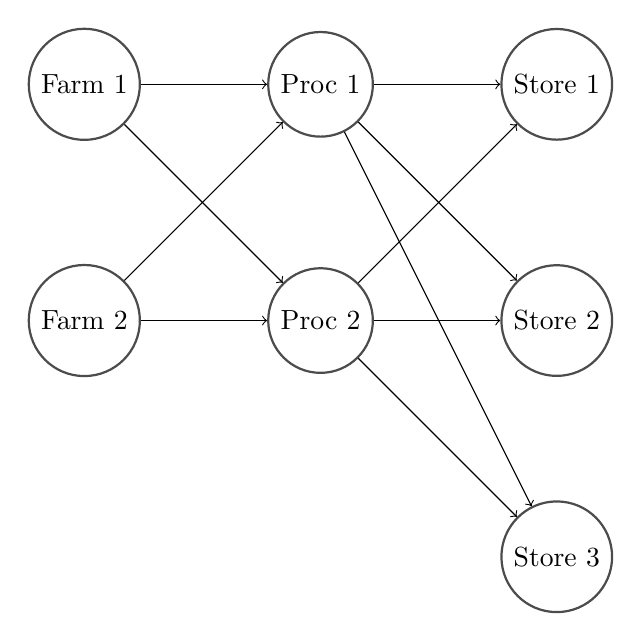
\begin{tikzpicture}[
node/.style={circle, draw=black!70, fill=white!5,  thick, minimum size=9mm}
]
%Nodes
\node[node]      (f1)                                        {Farm 1};
\node[node]      (f2)     [below of = f1, yshift= -2cm]       {Farm 2};
\node[node]      (p1)    [right of = f1, xshift= 2cm]        {Proc 1};
\node[node]      (p2)     [below of =p1, yshift= -2cm]       {Proc 2};
\node[node]      (s1)     [right of = p1 , xshift= 2cm]       {Store 1};
\node[node]      (s2)     [below of = s1, yshift= -2cm]       {Store 2};
\node[node]      (s3)     [below of = s2, yshift= -2cm]      {Store 3};
%Lines
\draw[->] (f1) -- (p1) ;%node [midway, fill=white] {};
\draw[->] (f1) -- (p2) ;%node [near start, fill=white] {};
\draw[->] (f2) -- (p1) ;%node [near start, fill=white] {distance};
\draw[->] (f2) -- (p2) ;%node [midway, fill=white] {distance};
\draw[->] (p1) -- (s1) ;%node [midway, fill=white] {distance};
\draw[->] (p1) -- (s2) ;%node [near start, fill=white] {distance};
\draw[->] (p1) -- (s3) ;%node [near end, fill=white] {distance};
\draw[->] (p2) -- (s1) ;%node [near end, fill=white] {distance};
\draw[->] (p2) -- (s2) ;%node [midway, fill=white] {distance};
\draw[->] (p2) -- (s3) ;%node [near start, fill=white] {distance};
\end{tikzpicture}
\caption{This figure shows the structure of the agricultural supply network in my model. Farms grow crops and send their product to intermediate processors. Processors send their product to stores. The processors and farms send their product to the next step in the network using local roads. They choose where to send their crops by minimizing costs.}
\label{fig:spec}
\end{framed}
\end{figure}

\section{Dual Problem}

Every linear problem can be stated two different ways as a primal and dual problem. In the dual version of a linear program, the constraints are used to construct new variables and the old variables are used to construct constraints. You turn the constraints into variables in order to increase their value as high as possible while maintaining the structure of the original primal problem. In the previous section, I described the primal version of optimal transport. I will now explain the second, dual way of looking at the problem. The dual is relevant to my project because I use it to calculate the transportation costs faced by suppliers. However, for the rest of the section, I will refer to transportation costs produced by calculating the dual variables as prices. In other words, when I mention prices in this section, I am not talking about the prices consumers face. 

It helps to think about the optimization variables in the dual problem as the prices producers pay to send goods through the network. These prices give firms incentive to send their goods along the optimal path. In the objective, firms try to maximize revenue made selling the good at demand nodes for $p_d$ but subtract the cost $p_s$ incurred by buying it from supply nodes.  

$$\operatorname{Maximize} \sum_{d \in D}  (\text{demand at } d) \cdot p_{d} -   \sum_{s \in S}  (\text{supply at } s) \cdot p_{s} $$

The prices incentivize the minimum-cost flow by discouraging paths through the network with negative costs. Prices are actually slack variables added into the problem when computing the costs of cycles. In other words, when you compute the costs of a cycle through the network by adding up the costs of each edge in the cycle, you add and subtract price $p$ at each node. Adding $p$ does not change how costly the cycle was. As long as the slack variables cancel out you are left with the cost of traveling through cycle. You use the slack variables to represent the reduced cost of moving between nodes. In other words, given $p_d$ is the price at demand node $d$ and $p_s$ is the price at supply node $s$, $p_d - p_s$ represents the amount moving a unit of goods from $d$ to $s$ reduces the total costs. To find prices, we maximize these reduced costs accounting for the number of times each node is visited. 

The constraints in the dual problem reflect the fact that you can only reduce the cost across an edge so much. At a certain point, you must traverse an edge and incur a cost. The most you can reduce the cost of traversing from from supplier $s$ to demand $d$ is the edge cost between the two, $c_{s,d}$. You can think about the constraints using the price metaphor. Firms $s$ earns $p_d$ for sending their product to $d$ and have to pay $p_s + c_{s,w}$ to get it there. In other words, the constraints say that the price at the source plus the edge cost must outweigh the cost at the destination. This prevents arbitrage through the network.

$$ p_d -p_s  \leq c_{s,d}$$

So, putting it all together we have formalized our dual problem:

$$\operatorname{Maximize} \sum_{d \in D}  (\text{demand at } d) \cdot p_{d} -   \sum_{s \in S}  (\text{supply at } s) \cdot p_{s} $$
$$ \text{ subject to}$$
$$ -p_s + p_d \leq c_{s,d},  \text{ for all edges }  s,d\in \textrm{Routes}$$

%reduction
Of course as before, we have to modify the problem to reflect the inclusion of intermediaries. The dual problem's objective stays exactly the same as before. The intermediate processors have prices, but since they do not keep any product their prices do not effect the profits firms make by sending their goods through the network.

$$\operatorname{Maximize} \sum_{s \in S}  (\text{demand at } s) \cdot p_{s} -   \sum_{f \in F}  (\text{supply at } f) \cdot p_{f} $$

Since, we added processors, we now need two sets of constraints. One reflects the cost of sending goods from farms to processors and another for the cost of sending goods between the processors and stores. These restrictions prevent every farm from sending their goods to a certain processor and processors from sending all their goods to a certain store.

$$ -p_f + p_p \leq c_{f,p}, \text{ for all edges }  f,p\in \textrm{Routes}$$
$$ -p_p + p_s \leq c_{p,s}, \text{ for all edges }  p,s\in \textrm{Routes}$$

Putting everything together we have our dual problem:

$$\operatorname{Maximize} \sum_{s \in S}  (\text{demand at } s) \cdot p_{s} -   \sum_{f \in F}  (\text{supply at } f) \cdot p_{f} $$
$$ \text{ subject to}$$
$$ -p_f + p_p \leq c_{f,p}, \text{ for all edges } f,p\in \textrm{Routes}$$
$$ -p_p + p_s \leq c_{p,s}, \text{ for all edges } p,s\in \textrm{Routes}$$


\chapter{Data Sources}

\section{Overview}

\section{Farms}

Because of the unique agricultural datasets New York state makes publicly available, I can estimate the transportation costs of moving produce from farms to stores using a linear program. New York state makes data regarding the supply chain of crops available. At the first step of the supply chain, I use data about the area and location of farms. Farms' production is proportional to their area. Since I chose a fairly small geographic region, soil, weather and other elements that effect the production of a crop will not vary greatly. The biggest difference affecting yields for farms is the area they dedicate to growing the crop. I can figure out farms' areas by looking at an image created by the National Agricultural Statistical Service \cite{nass}.

I use the pixels in a satellite image of crop cover to measure the size of farms. The data set is called the Cropland Data Layer and is created by measuring the way light reflects off the Earth at certain wavelengths using a satellite called Landsat. The satellite measures this reflection at thirty-by-thirty square meter plots. Based on the reflection is possible to classify point measured by the satellite. They are classified using using training data from the Farm Service Agency Common Land Unit Program. The file forms a grid called a raster where each pixel represents a certain crop band. The accuracy of classification for these pixels is individually poor. Table \ref{tab:band} conveys statistics about the satellite data's accuracy.

Although individual pixels may be unreliable, clusters of pixels correspond to the locations of farms. I used a technique called sieving to remove noise from the image. This technique involves identifying clusters of continuous pixels and dropping clusters of pixels that are too small. After putting the data through the sieve, I converted the raster file into vector based polygons. In the vector image, each cluster of continuous pixels became a farm for which I calculated an area and an centroid. To see what farms looked like across the various crops, I included Figure \ref{tab:farms}. You can see the distribution of farms and how their distribution related to the results in the appendix section.

\begin{table}[!t]
\centering
\begin{framed}
\begin{tabular}{c|c|c|c|c|c}%
	Crop&Band&Correct Pixels&Producer's Accuracy&Kappa&User's Accuracy
    \csvreader[head to column names, /csv/separator=semicolon]{band.csv}{}% use head of csv as column names
    {\\\hline \csvcoli & \csvcolii & \csvcoliii & \csvcoliv& \csvcolv & \csvcolvi}
\end{tabular}
\caption{This table shows the various errors associated with pixels in each crop band in the satellite image \cite{nass}. The statistics get determined by comparing the image with a small test set. Correct pixels are the number of pixels extrapolated from the training data. Producer's accuracy is a false negative, where pixels of a known crop are classified as something other than that crop. User's accuracy shows false positives, where pixels are incorrectly classified as a known crop when they should have been classified as something else. Kappa index of agreement gives an overall assessment of the accuracy of the classification.}
\label{tab:band}
\end{framed}
\end{table}


\begin{table}[!t]
\centering
\begin{framed}
\begin{tabular}{c|c|c|c|c|c}%
	Crop&Total Area&Average&Minimum&Maximum&Variance
    \csvreader[head to column names, /csv/separator=semicolon]{farms.csv}{}% use head of csv as column names
    {\\\hline \csvcoli & \csvcolii & \csvcoliii & \csvcoliv& \csvcolv & \csvcolvi}
\end{tabular}
\caption{This table summarizes some statistics of interest about the areas of farms. All areas are measured in square-meters. Onions take up the most area followed by grapes. Cabbages have the smallest range of sizes, but the highest variance within that range. Cherries have the smallest variance and the smallest total cover.}
\label{tab:farms}
\end{framed}
\end{table}

\section{Agricultural Dealers}

The next step in the supply chain are the intermediate processors. I included them for two reasons. They make the problem more realistic because farms do not sell their product directly to stores rather intermediaries.  More over, onions, cherries and cabbages are not exported or drastically changed during intermediate processing.  You need additional permits for to make processed foods. There may be an extra step of processing, but generally business with the necessary permits for processing buy in bulk directly from farms. The fact that only two of the three-hundred dealers were out of state reflects the self-contained nature of these markets. When onions, cherries or cabbages are sold to intermediate processors, they are going to be sold to stores in state due to the perishable nature of the crops. 

The second reason for including the intermediaries involves reducing the number of edges making the problem more computationally tractable. There were roughly three-hundred licensed agricultural product dealers in the data set. By forcing the edges between stores and farms to go through the processors, I drastically cut down the number of edges. 

In order to include intermediaries into the problem, I used the data on permits from the NYS Department of Agricultural Markets \cite{dam}. The state keeps a list of all the businesses that buy more than ten-thousand dollars in agricultural products. The data set had information about the crops they sold and their location as an address. I converted the addresses to spatial coordinates using Nominatim, an open source platform for geolocating. There are roughly three-hundred dealers but only half were relevant to my problem because they sold the right type of crop. I included Table \ref{tab:procs} to represent how many processors were associated with each crop. I did not have capacities on the agricultural dealers, but it seems reasonable to say the dealers could scale to accept as much product as farms want to send on the way to stores because they can scale.

\begin{table}[!t]
\centering
\begin{framed}
\begin{tabular}{c|c}%
	Crop & Count
    \csvreader[head to column names]{procs.csv}{}% use head of csv as column names
    {\\\hline \csvcoli & \csvcolii}
\end{tabular}
\caption{Grapes have the highest number of intermediaries associated with it. Cherries have the lowest number of intermediaries reflecting their seasonal nature.}
\label{tab:procs}
\end{framed}
\end{table}

%stores
\section{Stores}

The final step in the supply chain of onions, cherries, cabbages and grapes is stores. I do not know the exact amount of produce that makes it too this step. However, since Cabbages, cherries and onions production in New York is self contained because of these crops' limited shelf life and smaller scale production, I assume that the amount of produce in the state does not change from farms to stores. 

To estimate the amount of goods each stores sells, I use each stores size and nearby property values. I assume stores sell an amount proportional to their size weighted by property values. The weighted size reflects the fact that the amount a store sells is proportional to its fixed costs. Higher fixed costs mean the grocery stores need to sell more to recoup their investment. Although I do not have the exact fixed costs, the property makes up the majority of a stores' fixed cost. I can approximate the cost of their property by multiplying size by median property values. Intuitively, the median housing prices reflects the fact that a stores might have smaller square footage but higher turn-over. Stores in New York City might be the same size as a store upstate, but sell significantly more produce because the population density is much tighter in New York City and the consumers have more income to spend.

The data I used on stores came from NYS Division of Food Safety. It lists of stores that are given health inspections. The store data set has roughly twenty-thousand different stores and the classifications are based on their permits, their square footage and their GPS coordinates. I choose to look at the classification 'JAC' which are vendors that are registered as stores, manufacturers and multiple operations. This is because grocery stores fall under this category. Other categories were not as common and less relevant to selling fresh produce. I included a map of how they are spread through the state in Figure \ref{fig:map_3}. To get a sense of how the stores vary in size, I included Table \ref{tab:stores}.

So as not to have too many edges between the stores and the intermediaries, I aggregated the number of edges by Census tract. The reason for using this method of aggregations reflects the fact that median property values are measured at this level of granularity. Also, the census tracts for the most part represent municipalities. Two stores in the same town probably face the same demand for produce. You can see these weights in Figure \ref{fig:map_4}.


\begin{table}[!t]
\centering
\begin{framed}
\begin{tabular}{c|c|c|c}%
	Average&Minimum&Maximum&Variance
    \csvreader[head to column names, /csv/separator=semicolon]{stores.csv}{}% use head of csv as column names
    {\\\hline \csvcoli & \csvcolii & \csvcoliii & \csvcoliv}
\end{tabular}
\caption{This table conveys summary statistics about the characteristics of stores' square footage. Each of the columns are measured in square footage}
\label{tab:stores}
\end{framed}
\end{table}

\begin{sidewaysfigure}[!htb]
\centering
\begin{framed}
\includegraphics[scale=.50]{map_3}
\caption{Here I mapped all the stores as gray squares. They are over-layed on top of the census tracts so you can see how stores are spread out between them. You can see stores are much more sparsely spread in the center of the state.}
\label{fig:map_3}
\end{framed}
\end{sidewaysfigure}

\begin{sidewaysfigure}[!htb]
\centering
\begin{framed}
\includegraphics[scale=.50]{map_4}
\caption{This map shows the distribution of median housing values through out the census tracts. The darker the shading, the higher the median property value for that tract. You can see housing is cheap in western and northern New York, but expensive in the south western corners of the state.}
\label{fig:map_4}
\end{framed}
\end{sidewaysfigure}

\section{Edge Costs}

In order to connect each step in the supply chain, I created edges between each farm and processor and each processor and store. To measure the cost of moving the produce between farms, dealers and stores, I combine open source, publicly available maps of New York state's roads with open source routing software. The cost of traversing edge is expected travel time measured in seconds. For the crops I chose, travel times are an adequate measure of costs. These crops are grown on a small scale so roads are the best method for transporting the produce. The crops I analyze are being transported short enough distances in small enough quantities that I do not have to worry about a non-linear cost structure involved with transportation. The other factors involved with transporting produce like fuel, vehicle size and wages to drivers do not vary between suppliers on this scale. 

The open source software I use to measure travel times is called open source routing machine (OSRM). The algorithm that OSRM implements is called contraction hierarchies. It is a technique to speed up shortest-path routing by first creating precomputed 'contracted' versions of the connection graph. Contraction hierarchies can be used to generate shortest-path routes much more efficiently than the standard shortest path algorithm (i.e. Dijkstra's shortest path algorithm). I downloaded a map of New York from the open source mapping project (OSM) and answered routing queries over my local network. I included two tables to visualize the summary statistics of the edges. Table \ref{tab:fp_edges} shows the average, minimum, maximum and variance of edges between farms and product dealers. Table \ref{tab:ps_edges} shows the same for the edges between dealers and stores.


\begin{table}[!t]
\centering
\begin{framed}
\begin{tabular}{c|c|c|c|c}%
	Crop&Average&Minimum&Maximum&Variance
    \csvreader[head to column names, /csv/separator=semicolon]{fp_edges.csv}{}% use head of csv as column names
    {\\\hline \csvcoli & \csvcolii & \csvcoliii & \csvcoliv & \csvcolv}
\end{tabular}
\caption{This table conveys summary statistics about the characteristics of the edges between farms and agricultural product dealers. Grapes have the highest variability between edges. Each of the columns is measured in seconds of expected travel time}
\label{tab:fp_edges}
\end{framed}
\end{table}


\begin{table}[!t]
\centering
\begin{framed}
\begin{tabular}{c|c|c|c|c}%
	Crop&Average&Minimum&Maximum&Variance
    \csvreader[head to column names, /csv/separator=semicolon]{ps_edges.csv}{}% use head of csv as column names
    {\\\hline \csvcoli & \csvcolii & \csvcoliii & \csvcoliv & \csvcolv}
\end{tabular}
\caption{This table conveys summary statistics about the characteristics of the edges between farms and agricultural product dealers. The distances are similar to those of between farms and processors but they are less variable. Each of the columns is measured in seconds of expected travel time. }
\label{tab:ps_edges}
\end{framed}
\end{table}

\chapter{Results}

\section{Overview}

For my project, I asked how the network of farms, agricultural dealers and stores made fresh produce more expensive for consumers in certain areas. I used transportation costs to gain insight into where produce might be expensive. The small size of these markets ensures that transportation costs account for the major difference in the costs faced by firms. Demand is consistent between suppliers because prices are sticky and consumers and firms can move in the long run. As a result, its seems reasonable that transportation costs would indicate the actual prices consumers face. These costs are measured in travel times because wages, fuel prices and vehicle capacity are similar across the state. In order to estimate transportation costs, I tracked the movements of certain crops and estimated the cost by optimizing the movement of the crops through the network. The estimates assigns a cost to transporting produce at each point of interest in the network. In other words, farms, stores and processors all get assigned a transportation cost.

The most interesting part of the solution is the transportation costs at the store nodes. As you would expect, these estimates are highly related with the concentration of stores, house prices and the locations of farms. You can review the locations of stores and median house prices to reference their relation with the solution in Figures \ref{fig:map_3} and Figure \ref{fig:map_4}. In addition to stores, the farm and processor nodes also get assigned transportation costs. The transportation costs at the farms result when multiple stores want to receive crops from the same farm. For example, if a farm with a limited capacity has many stores nearby, you need to increase the price at that farm. This makes it less attractive for the nearby stores to ship produce from that farm. You can see an example of this in \ref{fig:prices_243}, the result of linear program for cabbages where farm prices are high.

According to the estimates, transportation costs at stores in western part of the state are low. This happened because farms are located in this region and the median house prices are low. There are a lot of farms and few stores. On the other hand, the south east and the northern corners of the state face significantly higher costs at stores. The south east faces the highest transportation costs for most crops because property values in this area are high and the concentration of farms is low. That the north would also be high in cost was surprising. Property values are low enough in this region to facilitate farming. Transportation costs are high here because the agricultural activities that take place are mostly focused on corn and dairy. The farms growing produce are also farthest from the state's northern regions. This is a troubling observation especially when you consider that this region also has lower median incomes compared to the rest of the state. It seems obvious that your distance from farms and property vales would increase transportation costs for fresh produce. The first reason for using the linear program to estimate transportation costs is that combines these datasets and describes their relationship in a quantifiable way.

Also, by estimating transportation costs through the network, certain observation about how the distribution of farms and stores effects costs emerge. Less obvious properties of the network can effect transportation costs. Specifically, variance in the size of farms gets amplified by the linear program. When you have fewer big farms, stores face bigger differences when choosing between farms. If the closest farm does not have enough capacity for all the nearby stores, then stores are forced to chose a farm that is further away incurring higher costs. When the farms vary in size, more stores are forced to chose between the closest farm and the second closest. As a result, costs are higher. I noticed this effect for cabbages where transportation costs are drastically higher than the other crops. On the other hand, when farm sizes vary less, so do costs as you can see for onions.

\section{Visualizing Results}

In many ways, the significance of the linear program is not obvious. It outputs a list of roughly eight-thousand transportation costs. In order to glean the key trends, I created tables that summarize statistics of result. Table  \ref{tab:price_49}, Table  \ref{tab:price_66}, Table  \ref{tab:price_69} and Table  \ref{tab:price_243} all show basic summary statistics about the mean and variance of the transportation costs in the linear program solution. Table \ref{tab:county_49}, Table \ref{tab:county_66}, Table \ref{tab:county_69} and Table \ref{tab:county_243} all summarize the range of possible transportation costs in the linear program for each of the crops I analyze. These tables summarize which counties have the highest and lowest transportation costs. As I said before, the counties in the west tend to have the lowest transportation costs. The counties in the south east tend to have the highest transportation costs, followed by the north. This is related to the locations of farms.

I also visualized the solution to the optimization problem over a map of New York state. I included them in the appendix because they each take up a page. They are vital to making the linear program intelligible. The first images shows the locations of farms based on the crop cover data that was put through the sieve. When you look at the pictures of farms, it becomes obvious how they influenced the solution. Areas around the farms have lower transportation costs. Additionally, the differences in the solutions related to the farms are more apparent because the stores and dealers stay roughly the same between the crops. The second map for each crop shows the locations of the farms, stores and dealers on the same map. Farms are represented by pentagons, dealers are stars and stores are squares. The final image I created for each crop visualizes the results of the linear program. It shows the various census tracts with shading based on the relative magnitude of the transportation costs. The number assigned to the price are most interesting in relation to each other.

%%%%%%%%%%%%%%%%%%%%%%%%%%%%%%%%%%%%%%%%%%%%%%%%%%%%%%%%%%%%%%%%%
%Descriptive Statistics 1 %%%%%%%%%%%%%%%%%%%%%%%%%%%%%%%%%%%%%%%
%%%%%%%%%%%%%%%%%%%%%%%%%%%%%%%%%%%%%%%%%%%%%%%%%%%%%%%%%%%%%%%%%

\begin{table}[!t]
\centering
\begin{framed}
\begin{tabular}{c|c|c|c}%
	Type&Average&Variance&Deviation
    \csvreader[head to column names, /csv/separator=semicolon]{price_49.csv}{}% use head of csv as column names
    {\\\hline \csvcoli & \csvcolii & \csvcoliii & \csvcoliv}
\end{tabular}
\caption{This table shows descriptive statistics about the transportation costs in the linear program for onions as measured in travel time. The transportation costs from the program represent travel time in seconds. You can see that onion farms are spread out enough that the program did not need to increase the price at the farms. The transportation costs at farms and processors get raised when multiple stores compete to buy onions from the same farm.}
\label{tab:price_49}
\end{framed}
\end{table}

\begin{table}[!t]
\centering
\begin{framed}
\begin{tabular}{c|c|c|c}%
	Type&Average&Variance&Deviation
    \csvreader[head to column names, /csv/separator=semicolon]{price_66.csv}{}% use head of csv as column names
    {\\\hline \csvcoli & \csvcolii & \csvcoliii & \csvcoliv}
\end{tabular}
\caption{This table shows descriptive statistics about the transportation costs in the linear program for cherries as measured in travel time. The cherry farms are small enough and spread apart enough that stores do not have to compete between sources. Stores can buy cherries from their most preferred farm. As a result, the transportation costs at farms is zero for all farms. Since there are less agricultural dealers that sell cherries and the farms are further from stores, the average transportation cost is higher when compared to the other crops.}
\label{tab:price_66}
\end{framed}
\end{table}


\begin{table}[!t]
\centering
\begin{framed}
\begin{tabular}{c|c|c|c}%
	Type&Average&Variance&Deviation
    \csvreader[head to column names, /csv/separator=semicolon]{price_69.csv}{}% use head of csv as column names
    {\\\hline \csvcoli & \csvcolii & \csvcoliii & \csvcoliv}
\end{tabular}
\caption{This table shows descriptive statistics about the transportation costs in the linear program as measured in travel time for grapes. You can see transportation costs at farms are transportation cost low, meaning farms are spread far enough apart so that stores do not have to compete over farms.}
\label{tab:price_69}
\end{framed}
\end{table}


\begin{table}[!t]
\centering
\begin{framed}
\begin{tabular}{c|c|c|c}%
	Type&Average&Variance&Deviation
    \csvreader[head to column names, /csv/separator=semicolon]{price_243.csv}{}% use head of csv as column names
    {\\\hline \csvcoli & \csvcolii & \csvcoliii & \csvcoliv}
\end{tabular}
\caption{This table shows descriptive statistics about the transportation costs in the linear program as measured in travel time for cabbages. The variance of the transportation costs is much higher than the other crops. Additionally, the cabbages are more expensive in the southeast in transportation cost affluent areas. For the other crops, prices were more expensive in the northwest. }
\label{tab:price_243}
\end{framed}
\end{table}


%%%%%%%%%%%%%%%%%%%%%%%%%%%%%%%%%%%%%%%%%%%%%%%%%%%%%%%%%%%%%%%
%Descriptive Statistics 2%%%%%%%%%%%%%%%%%%%%%%%%%%%%%%%%%%%%%%
%%%%%%%%%%%%%%%%%%%%%%%%%%%%%%%%%%%%%%%%%%%%%%%%%%%%%%%%%%%%%%%


\begin{table}[!t]
\centering
\begin{framed}
\begin{tabular}{c|c|c|c|c}%
	Type&Max Cost&Max County&Min Cost&Min County
    \csvreader[head to column names, /csv/separator=semicolon]{county_49.csv}{}% use head of csv as column names
    {\\\hline \csvcoli & \csvcolii & \csvcoliii & \csvcoliv & \csvcolv}
\end{tabular}
\caption{This table shows the minimum and maximum transportation cost for each step in the network according to the linear program for onions. The highest transportation costs were found in the northeast tip of the state (Clinton county). This area focuses on farming dairy and is far from the onion farms. The minimum transportation costs occur in the center by the most dense cluster of farms. You would expect prices to be higher for onions where transportation costs are high.}
\label{tab:county_49}
\end{framed}
\end{table}


\begin{table}[!t]
\centering
\begin{framed}
\begin{tabular}{c|c|c|c|c}%
	Type&Max Cost&Max County&Min Cost&Min County
    \csvreader[head to column names, /csv/separator=semicolon]{county_66.csv}{}% use head of csv as column names
    {\\\hline \csvcoli & \csvcolii & \csvcoliii & \csvcoliv & \csvcolv}
\end{tabular}
\caption{This table shows the minimum and maximum transportation costs and the counties that they occur for cherries. Like we saw in Table \ref{tab:price_66}, the minimum and maximum transportation cost at cherry farms is zero because stores do not want to import cherries from the same farms.  Multiple nodes in multiple counties have zero transportation costs at farms and processors. Transportation costs are highest in the northern counties of the state (Clinton county) because these counties focus on other types of agriculture. As always, transportation costs are measured in travel time in seconds.}
\label{tab:county_66}
\end{framed}
\end{table}

\section{Comparing Crops}

\begin{table}[!t]
\centering
\begin{framed}
\begin{tabular}{c|c|c|c|c}%
	Type&Max Cost&Max County&Min Cost&Min County
    \csvreader[head to column names, /csv/separator=semicolon]{county_69.csv}{}% use head of csv as column names
    {\\\hline \csvcoli & \csvcolii & \csvcoliii & \csvcoliv & \csvcolv}
\end{tabular}
\caption{This table shows the minimum and maximum transportation costs and the counties in which they occur for grapes. The transportation cost being zero reflects the fact that certain processors and farms are uncontested. In other words, only one stores wants to buy grapes from that farm or processor. Multiple counties may have zero transportation costs at farms and processors. As always, transportation costs are measured in travel time in seconds.} 
\label{tab:county_69}
\end{framed}
\end{table}


\begin{table}[!t]
\centering
\begin{framed}
\begin{tabular}{c|c|c|c|c}%
	Type&Max Cost&Max County&Min Cost&Min County
    \csvreader[head to column names, /csv/separator=semicolon]{county_243.csv}{}% use head of csv as column names
    {\\\hline \csvcoli & \csvcolii & \csvcoliii & \csvcoliv & \csvcolv}
\end{tabular}
\caption{This table shows the minimum and maximum transportation costs and the counties that they occur for cabbages. Cabbages are most expensive in the south east (Suffolk county) due to high variance among farms' size. As always, transportation costs are measured in travel time in seconds.}
\label{tab:county_243}
\end{framed}
\end{table}

The differences between the results for each of the different crops is as interesting as the results. Onion transportation costs are unique because there was a cluster of farms in the southern part of the state causing transportation costs to be lower there compared to some of the other crops. In fact, onions have both the lowest transportation costs and the lowest variance among transportation costs. The farms are spread far enough apart that stores due not try to ship onions from the same farm.

In terms of the various crops, cherries are by far the smallest in terms of production because they are seasonal. Their production is focused in the western portion of the state. Transportation costs are cheapest by farms and most expensive at the southeastern and northeastern parts of the state.

The grape farms are concentrated in the southwestern part of the state. There are some farms in the center of the state and also eastern Long Island. I included this crop because I calculated the edge costs for the grape farms which takes a long time. I do not think that grapes are traded using this framework. The supply grown at farms is mostly turned into juices and wines in New York.

Cabbages ended up being the most visually interesting as you can see in \ref{fig:prices_243}. The variance in the transportation costs calculated is noticeably higher than any of the other crops as we can see in Table \ref{tab:price_243}. This result is more striking in Figure \ref{fig:prices_243}. This result is directly related to the location of the farms through out the state. Although cabbages are also farmed in the western portion of the state, they are more spread apart and their size is more variable. This result translates through the network creating huge disparities further away from the farms. The results are most striking in the southeast as you can see  in Figures \ref{fig:stores_243_49}, Figures \ref{fig:stores_243_66} and Figures \ref{fig:stores_243_69}. These images compared cabbages prices with the other crops for most of the state.

I created a series of tables to convey summary statistics side by side. I created Table \ref{tab:farm_price} to compare the transportation costs for farms, Table \ref{tab:proc_price} to compare the transportation costs for processors and Table \ref{tab:store_price} to compare the transportation costs for the various census tracts in each of the crops. Table \ref{tab:farm_county}, Table \ref{tab:proc_county} and Table \ref{tab:store_county} to compare the information on minimum and maximum counties between the crops at farms, dealers and stores.

%%%%%%%%%%%%%%%%%%%aggregate%%%%%%%%%%%%%%%%%%%%%%%%%%%

\begin{table}[!t]
\centering
\begin{framed}
\begin{tabular}{c|c|c|c}%
	Crop&Average&Variance&Deviation
    \csvreader[head to column names, /csv/separator=semicolon]{farm_price.csv}{}% use head of csv as column names
    {\\\hline \csvcoli & \csvcolii & \csvcoliii & \csvcoliv}
\end{tabular}
\caption{This table compares the various transportation costs for the different farms in one place as measured in travel time. The transportation costs at farms encourage stores to ship produce from more remote farms. Transportation costs are lowest at cherry farms because stores are not requesting cherries from the same farm. The next lowest transportation costs are at onion farms. Transportation costs have the highest variance from the cabbage farms meaning certain farms are very popular with stores due to proximity. There are more cabbage farms spread out over the western portion of the state. This means that all the eastern stores want to import produce from the central counties (Onondaga county). As a result, the transportation cost needs to be increased to disincentive stores from ordering produce from these farms.}
\label{tab:farm_price}
\end{framed}
\end{table}


\begin{table}[!t]
\centering
\begin{framed}
\begin{tabular}{c|c|c|c}%
	Crop&Average&Variance&Deviation
    \csvreader[head to column names, /csv/separator=semicolon]{proc_price.csv}{}% use head of csv as column names
    {\\\hline \csvcoli & \csvcolii & \csvcoliii & \csvcoliv}
\end{tabular}
\caption{This table compares the transportation costs for the different agricultural dealers across the four crops in one place as measured in expected travel time. Cabbages have the highest transportation cost reflecting the similarly high transportation cost at farms. The transportation costs at the dealers reflects transportation costs at farms. Cabbages have high transportation costs at dealers reflecting the westward spread of farms.  Grapes have the highest variance reflecting the dense distribution of farms on the southwestern part of the state. Processors in this region have similarly disparate transportation costs when compared. }
\label{tab:proc_price}
\end{framed}
\end{table}


\begin{table}[!t]
\centering
\begin{framed}
\begin{tabular}{c|c|c|c}%
	Crop&Average&Variance&Deviation
    \csvreader[head to column names, /csv/separator=semicolon]{store_price.csv}{}% use head of csv as column names
    {\\\hline \csvcoli & \csvcolii & \csvcoliii & \csvcoliv}
\end{tabular}
\caption{This table compares the various descriptive statistics for the different stores across the four crops in one place. Cabbage farms are the most expensive. This reflects the fact the farms have less capacity and are not centralized. The high variance amplifies the expense for sending cabbages to the southeast (Suffolk county). Onions have the lowest price and the lowest variance followed by cherries, then grapes. }
\label{tab:store_price}
\end{framed}
\end{table}

\section{Robustness of Solutions}

%%%%%%%%%%%%%%%%%%%aggregate%%%%%%%%%%%%%%%%%%%%%%%%%%%

\begin{table}[!t]
\centering
\begin{framed}
\begin{tabular}{c|c|c|c|c}%
	Crop&Max Cost&Max County&Min Cost&Min County
    \csvreader[head to column names, /csv/separator=semicolon]{farm_county.csv}{}% use head of csv as column names
    {\\\hline \csvcoli & \csvcolii & \csvcoliii & \csvcoliv & \csvcolv}
\end{tabular}
\caption{This table compares the minimum and maximum transportation costs between the four crops for farms. The transportation costs reflect expected travel times. Cherry farms have the cheapest transportation costs followed by onions. Cabbages have the highest. This reflects the variance among the size of farms. Many stores want to import cabbages from the middle of the state. The variance in the size of farms is amplified through the network.}
\label{tab:farm_county}
\end{framed}
\end{table}

\begin{table}[!t]
\centering
\begin{framed}
\begin{tabular}{c|c|c|c|c}%
	Crop&Max Cost&Max County&Min Cost&Min County
    \csvreader[head to column names, /csv/separator=semicolon]{proc_county.csv}{}% use head of csv as column names
    {\\\hline \csvcoli & \csvcolii & \csvcoliii & \csvcoliv & \csvcolv}
\end{tabular}
\caption{This table compares the minimum and maximum transportation costs between the four crops for the agricultural dealers. The transportation costs reflect expected travel times. Again cabbages have the highest variance. }
\label{tab:proc_county}
\end{framed}
\end{table}


\begin{table}[!t]
\centering
\begin{framed}
\begin{tabular}{c|c|c|c|c}%
	Crop&Max Cost&Max County&Min Cost&Min County
    \csvreader[head to column names, /csv/separator=semicolon]{store_county.csv}{}% use head of csv as column names
    {\\\hline \csvcoli & \csvcolii & \csvcoliii & \csvcoliv & \csvcolv}
\end{tabular}
\caption{This table compares the minimum and maximum transportation costs between the four crops for the different census tracts. The transportation costs reflect expected travel times. Transportation costs are highest for cabbages and also exhibit the most variance. Transportation costs are highest for cabbages in the southeast (Suffolk county). Onions transportation costs are the lowest and also the most evenly distributed. }
\label{tab:store_county}
\end{framed}
\end{table}


%complementary slackness
One might be skeptical of any solution of this problem found by the simplex algorithm. Optimal transportation can have more than one possible solution. The example I worked out has more than one solution and I demonstrated it in Figure \ref{fig:example6}. The question becomes what other solutions exist to the problem and what properties persist through other optimal solutions. 

You can characterize all possible solutions to a linear program using a property is called complementary slackness. This property requires that the optimal value of the primal and the dual objective functions will be equivalent. The intuition behind this idea is straightforward to show with some matrix algebra.

Generally speaking a linear program has the primal form

$$\text{Maximize } c' x$$
$$\text{Subject to}$$
$$Ax \leq b$$

And, its corresponding dual would be

$$\text{Minimize } y' b$$
$$\text{Subject to}$$
$$A'y \leq c$$

We can modify the objective function to see that the values of the primal and dual objective functions will be the same

$$(A'y)' \leq c'$$
$$ y'A \leq c'$$
$$ y'Ax \leq c'x$$
$$y' b \leq c'x$$

In the same vain, 

$$ Ax \leq b$$
$$ y'Ax \leq y'b$$
$$ (yA')'x \leq c'x$$
$$ c'x \leq  y' b $$

As consequence of these two observations we know the objective functions must take the same value.

$$c'x = y' b$$

By this logic the objective function for any solution to the primal or dual problem will be the same. You can use this idea to check how robust certain properties of your solution are by adding the the optimal value of the objective function as a constraint. For example, you can test whether the maximum transportation cost $p = p^{max}$ only exists in your solution, by adding constraint extra constraints to your original problem. You add a constraint to limit the value of your objective function to be optimal. If the value of the objective was $c^*$ then you can add the constraint  $ \sum_{d \in D}  (\text{demand at } d) \cdot p_{d} -   \sum_{s \in S}  (\text{supply at } s) \cdot p_{s} = c^*$. Then you can try to change the transportation cost to see if can exceed the maximum by adding the constraint $p > p^{max}$.

For each of the crops, I tried to find an alternate solutions to the linear program in four ways using complementary slackness. I added constraints to make the maximum transportation cost higher or lower than in the original solution. I did the same thing with the minimum transportation cost. I was able get a second solution across all crops. This means my solution is not unique. Still, the differences were not drastic and the most obvious characteristics of the solution remained unchanged. In fact, in each file at most five-hundred of the roughly eight-thousand transportation costs across farms and stores changed. Most importantly the minimum and maximum values did not change by more than ten percent. I can provide the differences upon request. They can also be generated using my repository. They are rather cumbersome.

Changes in the solution have more to do with rounding errors related to the way that python stores floating point numbers rather than actual differences in the solution. When the value of the objective function is parsed from the solution files into python, floating points in the last significant digit are not accurate. This would explain differences in solutions.

\chapter{Conclusion}

\section{Discussion}

My project infers the different costs to stores of transporting certain types of produce from the supply chain. Ideally, these costs provide insight into general produce prices and nutritional outcomes. In order to argue that transportation costs determine prices, I argue stores face the same demand, factor costs and technology. Whether demand may vary is controversial. Like the rest of the literature on food deserts, my analysis stops short of relating the characteristics I discovered about supply to consumer behavior. For example, poor nutritional outcomes might discourage stores from building in a certain area. Transportation costs for these stores may be the same level as the rest of the network causing these areas to be overlooked.

I argue that I can overlook consumer behavior because prices are sticky in the short run and over the long term being near stores is less important. It seems reasonable that over long periods of time, consumers can move closer to stores that better serve their needs. More over, stores can change size and location to more evenly distribute demand. However, this assumption contradicts the food deserts literature which assumes that demand for produce in the city is not accommodated by nearby stores. Of course, access to produce on the scale of a city is different than access to produce on the scale of the state. My project looks at the state where there is more mobility.

Even without thinking about how consumers interact with transportation costs, the estimates I made are interesting. Estimating costs in the transportation network reveals observations about how the distribution of farms and stores effects costs are interesting from an industrial organization perspective. Additionally although consumer behavior determines price, the transportation costs are still relevant. These observations are useful to at least focus the scope of future investigations that consider how consumer behavior interacts with the size and placement of stores.  Relating consumer behavior to the network of food supply is an exciting avenue for future research.

Regardless of their relationship with consumer behavior, you can criticize the transportation costs because they do not represent suppliers' total costs. I argue that the self-contained nature of the problem means transportation costs represent biggest difference between suppliers of onions, cherries, grapes and cabbages. However, the stores are not as self contained as ideal. A lot of these stores are part of national chains. Perhaps decisions that are optimal for the business on a national scale do not seem optimal on a local level in terms of which farms and dealers the store decides to get its produce from. For example, one grocery chain might decide to work with only one agricultural dealer even though from the perspective of transportation costs, it would be beneficial to work with two. Also, although I tried chose a variety of crops, I may not have chosen enough to generalize my findings to other types of produce.

You can also criticize my specification of the problem. The crop production may not be contained to New York state. For example, the grape data is not informative because grapes are mostly processed. That being said, the estimated prices are still economically significant without exports. They represent a minimum for costs. Adding additional demand from out-of-state increases costs in-state. You could also argue data I used is misspecified. Census data about median house prices is not available for certain census tracts. There are always problems with classifying crops using satellite crops. There might be smaller farm dealers that do not register with the Department of Agricultural Markets because they sell less than ten-thousand dollars a year in goods. This would change the nature of the network. Still, data is never perfect. No mater what data I used, I could make improvements. Despite these reservations, the data paints a surprisingly detailed picture of agricultural markets in New York for onions, cherries, grapes, and cabbage. 


\section{Summary}

Despite my project's shortcomings, it improves the existing literature regarding food deserts by expanding the geographic scale and depth of considerations involved with identifying areas where produce is expensive. Although predicting prices through transportation costs seems circuitous, it offers the best possible insight into prices for produce on the scale of the state considering stores have incentive to keep data about state wide prices private. Optimal transportation also applies surprisingly well to explain how certain types of produce move through the supply chain considering the data available in New York. Producers face similar input costs so transportation costs are important in determining prices.

Depending upon how transportation costs interact with consumer behavior, the implications of this project are large. Since transporting food to the northeast and southeastern corners of the state is difficult one might worry about nutritional outcomes in those regions. More expensive prices on Long Island and New York city reflects the higher cost of living in those areas. However, the observations about the northern tip of the state are troubling. If transportation costs influence prices then it raises alarm about areas with high costs in the northern parts of the state. These regions have low median incomes, but high costs.

More over, transportation cost for produce are interesting from an industrial organization perspective. By estimating transportation costs through the network, certain observation about how the distribution of farms and stores effects costs emerge. Less obvious properties of the network can effect transportation costs. Specifically, variance in the size of farms gets amplified by the linear program. When you have fewer big farms, stores face bigger differences when choosing between farms.


\pagebreak

\begin{thebibliography}{99}
\bibitem{barrett}Barrett, C. (2010). Measuring Food Insecurity. Science, 327(5967), new series, 825-828. Retrieved from \url{http://www.jstor.org/stable/40509899}
\bibitem{Bernell}Bernell, S., Weber, B., {\&} Edwards, M. (2006). Restricted Opportunities, Personal Choices, Ineffective Policies: What Explains Food Insecurity in Oregon? Journal of Agricultural and Resource Economics, 31(2), 193-211. 
\bibitem{Chung} Chung, Chanjin and Samuel L. Myers. 'Do the Poor Pay More for Food? An Analysis of Grocery Store Availability and Food Price Disparities.' The Journal of Consumer Affairs 33.2 (1999): 276-96.
\bibitem{Cook} Cook, W. J., Cunningham, W. H., Pulleyblank, W. R.,  {\&}  Schrijver, A. (1998). Combinatorial optimization (pp. 91-126). New York: John Wiley  {\&}  Sons.
\bibitem{Hwang} Hwang, M., {\&} Smith, M. (2012). Integrating publicly available web mapping tools for cartographic visualization of community food insecurity: A prototype. GeoJournal, 77(1), 47-62.
\bibitem{Just} Just, R., {\&} Weninger, Q. (1997). Economic Evaluation of the Farmers' Market Nutrition Program. American Journal of Agricultural Economics, 79(3), 902-917.
\bibitem{dfs} NYS Division of Food Safety {\&} Inspection (2016). Retail Food Stores [Download table]. Retrieved from \url{https://data.ny.gov/Economic-Development/Retail-Food-Stores/9a8c-vfzj}
\bibitem{dam} NYS Department of Agriculture and Markets (DAM) (2016). Farm Product Dealer Licenses Currently Issued [Download table]. Retrieved from \url{https://data.ny.gov/Economic-Development/Retail-Food-Stores/9a8c-vfzj}
\bibitem{Larson} Larson, J., {\&} Moseley, W. (2012). Reaching the limits: A geographic approach for understanding food insecurity and household hunger mitigation strategies in Minneapolis-Saint Paul, USA. GeoJournal, 77(1), 1-12.
\bibitem{Stewart} Stewart, T., {\&} Ittmann, H. (1979). Two-Stage Optimization in a Transportation Problem. The Journal of the Operational Research Society, 30(10), 897-904.
\bibitem{census} U.S. Census Bureau. (2011). American Community Survey, 2010 ACS 5-year Selected Population Tables [Table B25077]. Retrieved from \url{https://factfinder.census.gov/faces/nav/jsf/pages/download_center.xhtml}
\bibitem{nass3} USDA, NASS. (2012) Census Publications Market Value of Ag Products. Retrieved from \url{https://www.agcensus.usda.gov/Publications/2012/Online_Resources/Rankings_of_Market_Value/New_York/}
\bibitem{nass} USDA, NASS. (2011). USDA National Agricultural Statistics Service 2010 New York Cropland Data Layer [Download]. Retrieved from \url{http://cugir.mannlib.cornell.edu/bucketinfo.jsp?id=8033}
\bibitem{nass2} USDA, NASS. (2015) QuickStat Searchable Database. [New York state, Fruit and Tree Nuts, Vegetables, Cherries, Onions, Cabbages, Grapes]. Retrieved from \url{https://www.nass.usda.gov/Statistics_by_State/New_York/}

\end{thebibliography}


\chapter{Appendix}

\section{Worked Out Optimal Transportation}

\begin{figure}[!htb]
\centering
\begin{framed}
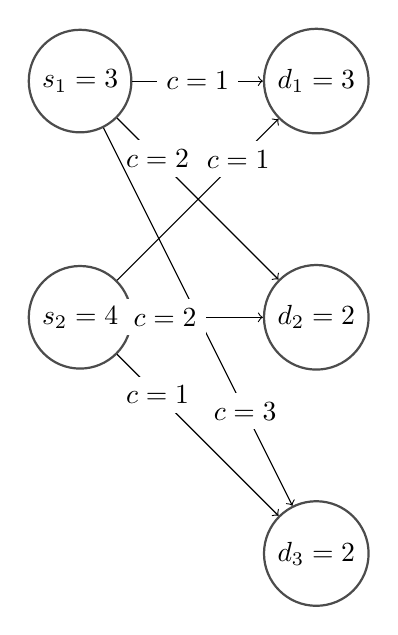
\begin{tikzpicture}[
node/.style={circle, draw=black!70, fill=white!5,  thick, minimum size=9mm}
]
%Nodes
\node[node]      (s1)                                        {$s_1= 3$};
\node[node]      (s2)     [below of =s1, yshift= -2cm]       {$s_2 = 4$};
\node[node]      (d1)     [right of =s1 , xshift= 2cm]       {$d_1 = 3$};
\node[node]      (d2)     [below of = d1, yshift= -2cm]       {$d_2 = 2$};
\node[node]      (d3)     [below of = d2, yshift= -2cm]      {$d_3 = 2$};
%Lines
\draw[->] (s1) -- (d1) node [midway, fill=white] {$c= 1$};
\draw[->] (s1) -- (d2) node [near start, fill=white] {$c = 2$};
\draw[->] (s1) -- (d3) node [near end, fill=white] {$c = 3$};
\draw[->] (s2) -- (d1) node [near end, fill=white] {$c = 1$};
\draw[->] (s2) -- (d2) node [near start, fill=white] {$c = 2$};
\draw[->] (s2) -- (d3) node [near start, fill=white] {$c = 1$};
\end{tikzpicture}
\caption{This picture represents the network for which we will be finding minimum-cost flow. The supply and demand nodes are labeled with their corresponding capacities.  The edges between each supply and demand nodes are labeled according to their cost. To make the problem easier, you can assume all edges have unlimited capacity meaning suppliers can send as much goods as they want over them.}
\label{fig:example1}
\end{framed}
\end{figure}

\begin{figure}[!htb]
\centering
\begin{framed}
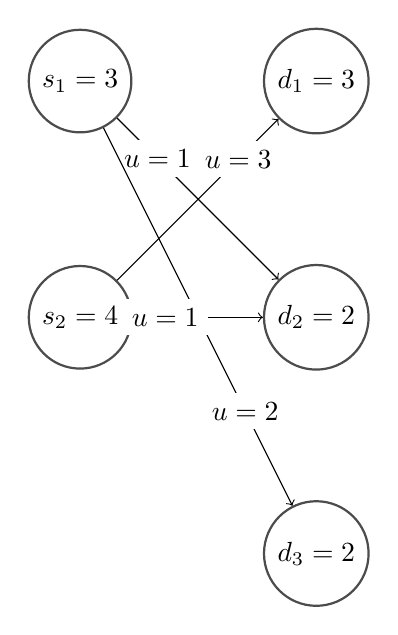
\begin{tikzpicture}[
node/.style={circle, draw=black!70, fill=white!5,  thick, minimum size=9mm}
]
%Nodes
\node[node]      (s1)                                        {$s_1= 3$};
\node[node]      (s2)     [below of =s1, yshift= -2cm]       {$s_2 = 4$};
\node[node]      (d1)     [right of =s1 , xshift= 2cm]       {$d_1 = 3$};
\node[node]      (d2)     [below of = d1, yshift= -2cm]       {$d_2 = 2$};
\node[node]      (d3)     [below of = d2, yshift= -2cm]      {$d_3 = 2$};
%Lines
\draw[->] (s1) -- (d2) node [near start, fill=white] {$u = 1$};
\draw[->] (s1) -- (d3) node [near end, fill=white] {$u = 2$};
\draw[->] (s2) -- (d1) node [near end, fill=white] {$u = 3$};
\draw[->] (s2) -- (d2) node [near start, fill=white] {$u = 1$};
\end{tikzpicture}
\caption{The algorithm starts by matching the capacities on the supply nodes with the capacities on the demand nodes. This is trivial because there are no edge capacities and every node is connected.}
\label{fig:example2}
\end{framed}
\end{figure}

\begin{figure}[!htb]
\centering
\begin{framed}
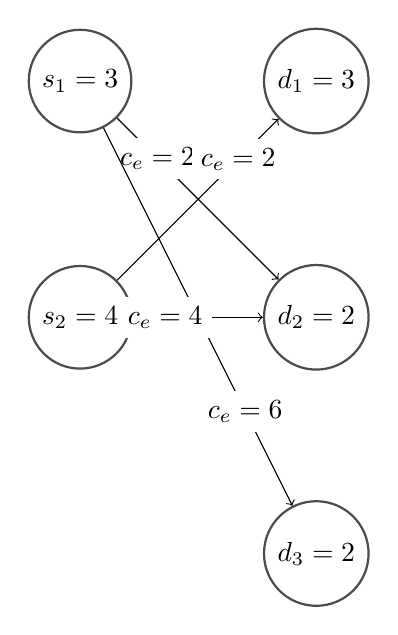
\begin{tikzpicture}[
node/.style={circle, draw=black!70, fill=white!5,  thick, minimum size=9mm}
]
%Nodes
\node[node]      (s1)                                        {$s_1= 3$};
\node[node]      (s2)     [below of =s1, yshift= -2cm]       {$s_2 = 4$};
\node[node]      (d1)     [right of =s1 , xshift= 2cm]       {$d_1 = 3$};
\node[node]      (d2)     [below of = d1, yshift= -2cm]       {$d_2 = 2$};
\node[node]      (d3)     [below of = d2, yshift= -2cm]      {$d_3 = 2$};
%Lines
\draw[->] (s1) -- (d2) node [near start, fill=white] {$c_e = 2$};
\draw[->] (s1) -- (d3) node [near end, fill=white] {$c_e = 6$};
\draw[->] (s2) -- (d1) node [near end, fill=white] {$c_e = 2$};
\draw[->] (s2) -- (d2) node [near start, fill=white] {$c_e = 4$};
\end{tikzpicture}
\caption{This solution is not optimal in terms of cost (yet). I labeled each edge in this figure with the cost each edge has incurred. It works out to 14. The edge costs are the amount of flow on each edge times its cost.}
\label{fig:example3}
\end{framed}
\end{figure}

\begin{figure}[!htb]
\centering
\begin{framed}
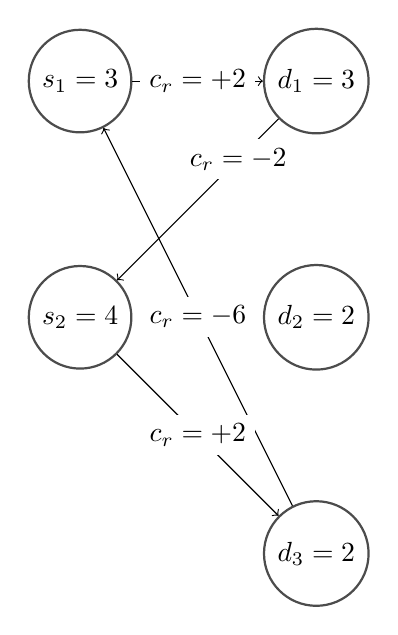
\begin{tikzpicture}[
node/.style={circle, draw=black!70, fill=white!5,  thick, minimum size=9mm}
]
%Nodes
\node[node]      (s1)                                        {$s_1= 3$};
\node[node]      (s2)     [below of =s1, yshift= -2cm]       {$s_2 = 4$};
\node[node]      (d1)     [right of =s1 , xshift= 2cm]       {$d_1 = 3$};
\node[node]      (d2)     [below of = d1, yshift= -2cm]       {$d_2 = 2$};
\node[node]      (d3)     [below of = d2, yshift= -2cm]      {$d_3 = 2$};
%Lines
\draw[->] (s1) -- (d1) node [midway, fill=white] {$c_r=+2$};
\draw[<-] (s1) -- (d3) node [midway, fill=white] {$c_r= -6$};
\draw[<-] (s2) -- (d1) node [near end, fill=white] {$c_r=-2 $};
\draw[->] (s2) -- (d3) node [midway, fill=white] {$c_r=+2$};
\end{tikzpicture}
\caption{In order to improve the cost of flow through the network, we look for a reduced cost cycle. The cycle needs to start and end on the same node. It also needs to alternate between suppliers and demand nodes. This is because you delete costly edges and replace them with less expensive ones. By traversing the cycle we see can reduce the cost by 4 to the optimal amount. Edges in the cycle are labeled with their reduced cost (i.e. how much they improve the total cost)}
\label{fig:example4}
\end{framed}
\end{figure}

\begin{figure}[!htb]
\centering
\begin{framed}
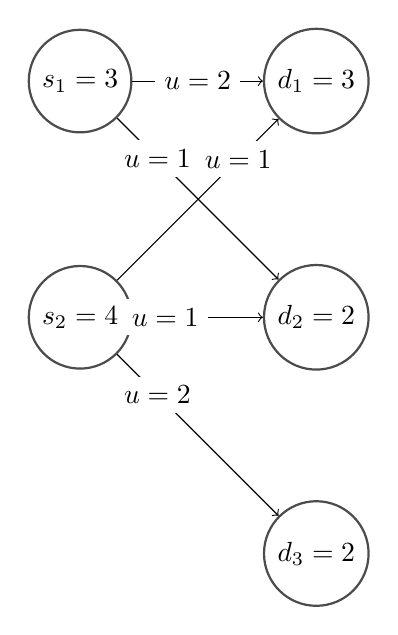
\begin{tikzpicture}[
node/.style={circle, draw=black!70, fill=white!5,  thick, minimum size=9mm}
]
%Nodes
\node[node]      (s1)                                        {$s_1= 3$};
\node[node]      (s2)     [below of =s1, yshift= -2cm]       {$s_2 = 4$};
\node[node]      (d1)     [right of =s1 , xshift= 2cm]       {$d_1 = 3$};
\node[node]      (d2)     [below of = d1, yshift= -2cm]       {$d_2 = 2$};
\node[node]      (d3)     [below of = d2, yshift= -2cm]      {$d_3 = 2$};
%Lines
\draw[->] (s1) -- (d1) node [midway, fill=white] {$u=2$};
\draw[->] (s1) -- (d2) node [near start, fill=white] {$u=1$};
\draw[->] (s2) -- (d1) node [near end, fill=white] {$u=1$};
\draw[->] (s2) -- (d2) node [near start, fill=white] {$u=1$};
\draw[->] (s2) -- (d3) node [near start, fill=white] {$u=2$};
\end{tikzpicture}
\caption{At this point, there are no more reduced cost cycles, so we found an optimal solution in terms of cost. The edges reflect the amount of units flowing from supply to demand in this solution.}
\label{fig:example5}
\end{framed}
\end{figure}

\begin{figure}[!t]
\centering
\begin{framed}
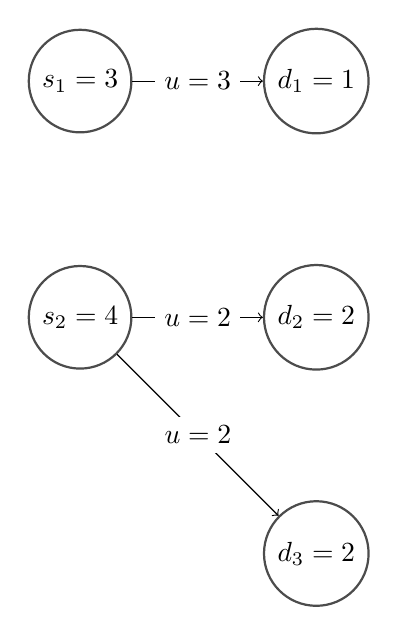
\begin{tikzpicture}[
node/.style={circle, draw=black!70, fill=white!5,  thick, minimum size=9mm}
]
%Nodes
\node[node]      (s1)                                        {$s_1= 3$};
\node[node]      (s2)     [below of =s1, yshift= -2cm]       {$s_2 = 4$};
\node[node]      (d1)     [right of =s1 , xshift= 2cm]       {$d_1 = 1$};
\node[node]      (d2)     [below of = d1, yshift= -2cm]       {$d_2 = 2$};
\node[node]      (d3)     [below of = d2, yshift= -2cm]      {$d_3 = 2$};
%Lines
\draw[->] (s1) -- (d1) node [midway, fill=white] {$u=3$};
\draw[->] (s2) -- (d2) node [midway, fill=white] {$u=2$};
\draw[->] (s2) -- (d3) node [midway, fill=white] {$u=2$};
\end{tikzpicture}
\caption{As long as there are no minimum-cost cycles we found a solution. Zero-cost cycles exists in this simple network. As a result, there is more than one solution that optimizes cost and flow. This figure shows that example.}
\label{fig:example6}
\end{framed}
\end{figure}

\section{Maps}

In this section, I visualize the solution to the optimization problem over a map of New York state. Figure \ref{fig:farms_49}, Figure \ref{fig:farms_66}, Figure \ref{fig:farms_69} and Figure \ref{fig:farms_243} show the location of farms for each of the respective crops. The locations of farms explain a lot about the differences between solutions. Figure \ref{fig:network_49}, Figure \ref{fig:network_66}, Figure \ref{fig:network_69} and Figure \ref{fig:network_243} show how the network looks for each of the respective crops. Stores and processors contribute to solution especially with regards to their location with respect to farms.  Figure \ref{fig:prices_49} , Figure \ref{fig:prices_66}, Figure \ref{fig:prices_69} and Figure \ref{fig:prices_243} all show how the network looks for each of the respective crops. These directly summarize where the linear program predicts produce to be expensive for each crop.

I also included three images comparing the transportation costs generated at the intermediaries by the linear program for cabbages to onions, cherries and grapes in Figures \ref{fig:procs_243_49}, Figures \ref{fig:procs_243_66} and Figures \ref{fig:procs_243_69}. Similarly, I also included three images comparing the transportation costs generated at the census tracts by the linear program for cabbages to onions, cherries and grapes in Figures \ref{fig:stores_243_49}, Figures \ref{fig:stores_243_66} and Figures \ref{fig:stores_243_69}.



%%%%%%%%%%%%%%%%%%%%%%%%%%%%%%%%%%%%%%%%%%%%%%%%%%%%%%%%%%%%%%%%%
%Farms%%%%%%%%%%%%%%%%%%%%%%%%%%%%%%%%%%%%%%%%%%%%%%%%%%%%%%%%%%%
%%%%%%%%%%%%%%%%%%%%%%%%%%%%%%%%%%%%%%%%%%%%%%%%%%%%%%%%%%%%%%%%%

\begin{sidewaysfigure}[!htb]
\centering
\begin{framed}
\includegraphics[scale=.50]{farms_49}
\caption{This figure shows the location of onion farms based on the cropland data put through the sieve. You can see there are roughly four clusters of farms. Three of them are in the center of the state and the fourth is south. The locations of farms influenced the prices. If you are interested in how this map relates to the descriptive statistics of the farms you can see Table \ref{tab:farms}.}
\label{fig:farms_49}
\end{framed}
\end{sidewaysfigure}

\begin{sidewaysfigure}[!htb]
\centering
\begin{framed}
\includegraphics[scale=.50]{farms_66}
\caption{This figure shows the location of cherry farms based on the cropland data put through the sieve. Cherries had the least amount of area dedicated to them and the farms were scattered throughout the far west portion of the state. As a result, the transportation costs for cherry are higher.}
\label{fig:farms_66}
\end{framed}
\end{sidewaysfigure}

\begin{sidewaysfigure}[!htb]
\centering
\begin{framed}
\includegraphics[scale=.50]{farms_69}
\caption{This figure shows the location of grape farms based on the cropland data put through the sieve. There is a dense band of farms in the south west portion of the state. There are smaller clusters in the south central part of the state and the northwest. }
\label{fig:farms_69}
\end{framed}
\end{sidewaysfigure}

\begin{sidewaysfigure}[!htb]
\centering
\begin{framed}
\includegraphics[scale=.50]{farms_243}
\caption{This figure shows the location of cabbage farms based on the cropland data put through the sieve. The cabbage farms are transportation cost spread out compared to the other crops.}
\label{fig:farms_243}
\end{framed}
\end{sidewaysfigure}

%%%%%%%%%%%%%%%%%%%%%%%%%%%%%%%%%%%%%%%%%%%%%%%%%%%%%%%%%%%%%%%%%
%Network%%%%%%%%%%%%%%%%%%%%%%%%%%%%%%%%%%%%%%%%%%%%%%%%%%%%%%%%%
%%%%%%%%%%%%%%%%%%%%%%%%%%%%%%%%%%%%%%%%%%%%%%%%%%%%%%%%%%%%%%%%%

\begin{sidewaysfigure}[!htb]
\centering
\begin{framed}
\includegraphics[scale=.50]{network_49}
\caption{This figure visualizes onion supply network in New York. The pentagons are farms, the stars are processors and the squares are stores. Onions had the second highest number of intermediate dealers to choose from as you can see in Table \ref{tab:procs}}
\label{fig:network_49}
\end{framed}
\end{sidewaysfigure}

\begin{sidewaysfigure}[!htb]
\centering
\begin{framed}
\includegraphics[scale=.50]{network_66}
\caption{This figure visualizes the cherries supply network in New York. The pentagons are farms, the stars are processors and the squares are stores. You can see how many dealers there were in the other table. The cherries had the least amount of dealers dedicated to them so prices are highest at the cherries.}
\label{fig:network_66}
\end{framed}
\end{sidewaysfigure}

\begin{sidewaysfigure}[!htb]
\centering
\begin{framed}
\includegraphics[scale=.50]{network_69}
\caption{This figure visualizes the grape supply network in New York. The pentagons are farms, the stars are processors and the squares are stores. }
\label{fig:network_69}
\end{framed}
\end{sidewaysfigure}

\begin{sidewaysfigure}[!htb]
\centering
\begin{framed}
\includegraphics[scale=.50]{network_243}
\caption{This figure visualizes the cabbage supply network in New York. The pentagons are farms, the stars are processors and the squares are stores.}
\label{fig:network_243}
\end{framed}
\end{sidewaysfigure}

%%%%%%%%%%%%%%%%%%%%%%%%%%%%%%%%%%%%%%%%%%%%%%%%%%%%%%%%%%%%%%%%%
%Prices%%%%%%%%%%%%%%%%%%%%%%%%%%%%%%%%%%%%%%%%%%%%%%%%%%%%%%%%%%
%%%%%%%%%%%%%%%%%%%%%%%%%%%%%%%%%%%%%%%%%%%%%%%%%%%%%%%%%%%%%%%%%

\begin{sidewaysfigure}[!htb]
\centering
\begin{framed}
\includegraphics[scale=.50]{prices_49}
\caption{This figure shows the distribution of onion prices through out the state according to the linear program. You can see that the prices are highest in the northeast and southeast corners of the state. The fact that there was a cluster of farms in the southern part of the state caused prices to be lower there compared to some of the other crops.}
\label{fig:prices_49}
\end{framed}
\end{sidewaysfigure}


\begin{sidewaysfigure}[!htb]
\centering
\begin{framed}
\includegraphics[scale=.50]{prices_66}
\caption{This figure shows the distribution of cherry prices through out the state according to the linear program. The darker the shading the higher the price. You can see that the prices are highest in the northeast and the southeast corners of the states. This reflects these regions relative distance from farms. Prices are high in the northern part of the state because this region focuses on other types of farming, mainly dairy. Prices are high in the south east because land in these areas is not used for farming. }
\label{fig:prices_66}
\end{framed}
\end{sidewaysfigure}


\begin{sidewaysfigure}[!htb]
\centering
\begin{framed}
\includegraphics[scale=.50]{prices_69}
\caption{This figure shows the distribution of grape prices through out the state according to the linear program. The darker the shading the higher the price. Because of the farms dense concentration on the western portion of the state, the prices in the west are consistently low when compared to the east. This means you would expect it to be less expensive to find grapes in the western portion of the state because transportation costs are lower.}
\label{fig:prices_69}
\end{framed}
\end{sidewaysfigure}


\begin{sidewaysfigure}[!htb]
\centering
\begin{framed}
\includegraphics[scale=.50]{prices_243}
\caption{This figure shows the distribution of cabbage prices through out the state according to the linear program. The darker the shading the higher the price. The result for cabbages seems more spread out across the state because of the shading grade. In actuality, the result was similar to the others. However, prices in the southeast are significantly higher for cabbages than the other crops. This variance causes the figure to look more evenly distributed than the other farms. The high prices in the south east reflect the locations of farms.}
\label{fig:prices_243}
\end{framed}
\end{sidewaysfigure}


%%%%%%%%%%%%%%%%%%%%%%%%%%%%%%%%%%%%%%%%%%%%%%%%%%%%%%%%%%%%%%%%%
%price Differences%%%%%%%%%%%%%%%%%%%%%%%%%%%%%%%%%%%%%%%%%%%%%%%
%%%%%%%%%%%%%%%%%%%%%%%%%%%%%%%%%%%%%%%%%%%%%%%%%%%%%%%%%%%%%%%%%

\begin{sidewaysfigure}[!htb]
\centering
\begin{framed}
\includegraphics[scale=.50]{procs_243_49}
\caption{This figure compares the difference in prices between onions and cabbages at the intermediaries. I chose cabbages because the result of the linear program was most different for this crop. The stars represent the dealers. Darker means onion prices were greater. Lighter means cabbage prices were greater.}
\label{fig:procs_243_49}
\end{framed}
\end{sidewaysfigure}

\begin{sidewaysfigure}[!htb]
\centering
\begin{framed}
\includegraphics[scale=.50]{procs_243_66}
\caption{This figure compares the difference in prices between cherries and cabbages at the intermediaries. I chose cabbages because the result of the linear program was most different for this crop. The stars represent the dealers. Darker means cherry prices were greater. Lighter means cabbage prices were greater.}
\label{fig:procs_243_66}
\end{framed}
\end{sidewaysfigure}

\begin{sidewaysfigure}[!htb]
\centering
\begin{framed}
\includegraphics[scale=.50]{procs_243_69}
\caption{This figure compares the difference in prices between grapes and cabbages at the intermediaries. I chose cabbages because the result of the linear program was most different for this crop. The stars represent the dealers. Darker means grape prices were greater. Lighter means cabbage prices were greater.}
\label{fig:procs_243_69}
\end{framed}
\end{sidewaysfigure}

\begin{sidewaysfigure}[!htb]
\centering
\begin{framed}
\includegraphics[scale=.50]{stores_243_49}
\caption{This figure compares the difference in prices between onions and cabbages at the census tracts. I chose cabbages because the result of the linear program was most different for this crop. The stars represent the dealers. Darker means onion prices were greater. Lighter means cabbage prices were greater.}
\label{fig:stores_243_49}
\end{framed}
\end{sidewaysfigure}

\begin{sidewaysfigure}[!htb]
\centering
\begin{framed}
\includegraphics[scale=.50]{stores_243_66}
\caption{This figure compares the difference in prices between cherries and cabbages at the census tracts. I chose cabbages because the result of the linear program was most different for this crop. The stars represent the dealers. Darker means cherry prices were greater. Lighter means cabbage prices were greater.}
\label{fig:stores_243_66}
\end{framed}
\end{sidewaysfigure}

\begin{sidewaysfigure}[!htb]
\centering
\begin{framed}
\includegraphics[scale=.50]{stores_243_69}
\caption{This figure compares the difference in prices between grapes and cabbages at the census tracts. I chose cabbages because the result of the linear program was most different for this crop. The stars represent the dealers. Darker means grape prices were greater. Lighter means cabbage prices were greater.}
\label{fig:stores_243_69}
\end{framed}
\end{sidewaysfigure}


\end{document}